\problemname{Flower Cutting}

In the CEOI community garden, we are growing a collection of special flowers
that tightly knit their roots together. If we cut them, they regrow, as long as
we do not cut too aggressively and cause irreparable damage.

If a pair of flowers, $a$ and $b$, knit their roots together, we call them
``connected''. Otherwise, they are ``disconnected''. Roots grow according to the
following rule: Let $a$ and $b$ be two disconnected flowers. If at least $2$
other flowers $c$ and $d$ exist, such that each of $a$ and $b$ is connected with
both $c$ and $d$, then roots between $a$ and $b$ will grow, and they will become
connected.

These flowers have now been growing for a while, and all the roots that could
grow by following the above rule have grown. In other words, if two flowers $a$
and $b$ are both connected with some flowers $c$ and $d$, then $a$ and $b$ are
guaranteed to be connected with each other.

We need to uproot this garden and move it to the next CEOI location. To simplify
the migration, we would like to cut as many roots as possible. However, we want
the flowers to regrow back into their current state. What is the maximum number
of connected pairs of flowers that we may cut so that they still regrow back
into their current state? It does not matter how many iterations of growth it
would take.

\section*{Input}
The first line of the input contains two space-separated integers $n$ and $m$,
the number of flowers and the number of existing connections between them. This
is followed by $m$ lines, each containing a pair of integers $a_i$ and $b_i$,
indicating that flowers $a_i$ and $b_i$ are connected. Flowers are marked with
integers $1 \ldots n$. The input is guaranteed to follow the rule described in
the task description.

The following limits hold:
\begin{itemize}
  \item $1 \leq n \leq 1000$
  \item $1 \leq m \leq 10^5$
\end{itemize}

\section*{Output}
Output a single integer --- the maximum number of connections that we may cut.

\section*{Scoring}
Your solution will be tested on a set of test groups.
To earn points for a group, you must pass all test cases in that group.

\noindent
\begin{tabular}{| l | l | p{12cm} |}
  \hline
  \textbf{Group} & \textbf{Points} & \textbf{Constraints} \\ \hline
  $1$ & $20$ & $n \leq 10$ and $m \leq 20$ \\ \hline
  $2$ & $14$ & $m = \frac{n \cdot (n-1)}{2}$ \\ \hline
  $3$ & $15$ & We guarantee that each flower is connected with at most $7$ other
               flowers. \\ \hline
  $4$ & $15$ & $n \leq 50$ and $m \leq 1000$ \\ \hline
  $5$ & $36$ & No additional constraints. \\ \hline
\end{tabular}

\section*{Explanation of Samples}
% Plain `center` rather than `figure`: \caption* renders as a literal "Figure 1: *" in both
% the Kattis PDF and HTML output, and a floating `figure` migrates away from this section
% (with [htp] both illustrations landed a page above their own heading). A non-float keeps
% the caption text intact and the reading order fixed.
\begin{center}
  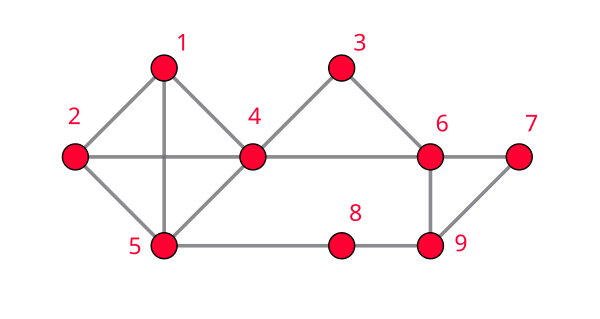
\includegraphics[width=0.55\textwidth]{flowers-1}

  \vspace{0.5cm}
  \parbox{\linewidth}{\centering
    The flowers in the example before any cutting. One can check that no
    additional connections can form based on the described growth procedure.
  }
\end{center}

\begin{center}
  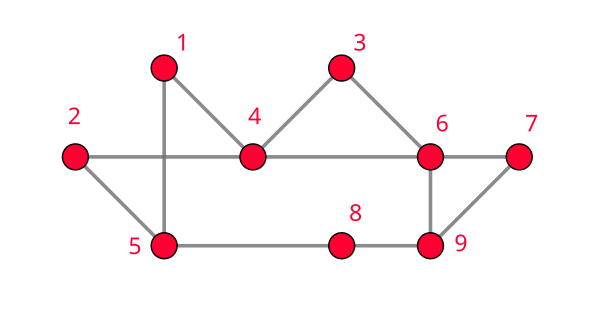
\includegraphics[width=0.55\textwidth]{flowers-2}

  \vspace{0.5cm}
  \parbox{\linewidth}{\centering
    The flowers in the example after the cutting have $2$ connections less. The
    connection between $1$ and $2$ can regrow because flowers $1$ and $2$ are
    both connected to flowers $4$ and $5$. Similarly, the connection between $4$
    and $5$ can regrow because flowers $4$ and $5$ are both connected to
    flowers $1$ and $2$.
  }
\end{center}
